\documentclass[english,12pt]{article}

\usepackage{enumitem}
\usepackage{tikz}
\usepackage{mlmodern}
\usepackage{pgfplots}
\usepackage{amssymb}
\usepackage{mathtools}
\usepackage{booktabs}
\usepackage{multirow}
\usepackage{siunitx}
\usepackage{subcaption}
\usepackage{amsmath}
\usepackage{enumerate}
\usepackage[american]{circuitikz-1.1.2}
\usepackage{bm}
\usepackage{graphicx}
\usepackage[margin=2cm]{geometry}
\usepackage{indentfirst}
\usepackage[english]{babel}
\usepackage[utf8]{inputenc}
\usepackage{fancyhdr}
\usepackage{tikz-feynman}
\usepackage{physics}
\usepackage{color}
\usepackage{siunitx}
\usepackage[style=apa,backend=biber]{biblatex}
\addbibresource{export.bib}
\renewcommand{\baselinestretch}{1.5}
\setlength{\parskip}{0.4cm}
\pagestyle{fancy}
\fancyhead{}
\fancyfoot{}
\usepackage{titlesec}
\titleformat{\section}
  {\normalfont\bfseries\Large}{\thesection}{1em}{}[{}]
\titleformat{\subsection}{\normalfont\bfseries}{\thesubsection}{1em}{}[]
  \usepackage{hyperref}
\hypersetup{
    colorlinks=true,
    linkcolor=blue,
    filecolor=magenta,      
    urlcolor=cyan,
    citecolor=blue,
    pdftitle={\writetitle PDF},
}
\fancyhead[l]{\fontsize{8}{12}\slshape\MakeUppercase{\writetitle}}
\fancyhead[R]{\slshape{\writename}}
\fancyfoot[c]{\thepage}
\pgfplotsset{compat=1.17}


%Configuration%
\newcommand{\ltspice}[]{\textit{LTSpice} }
    \newcommand{\writetitle}{Thévenin equivalent, Superposition circuits, and Voltage buffer}
    \newcommand{\writename}{Samuel Morales}
    \newcommand{\writesubtitle}{Section 004 (Zainab Imran)}

\begin{document}
\thispagestyle{plain}
	\begin{center}
	\hspace{0pt}
	{\large\textbf{{\writetitle}}}

    \writename
    
    \today
    
	\writesubtitle

\end{center}
\begin{abstract}
    In this experiment, the implementation of powerful circuit theorems is explored. The superposition principle and Thévenin equivalent theorem are proved with specific scenarios. The first one being a computer simulation using \ltspice, while the second one an actual circuit built in the lab. Also, the usage of a voltage buffer is implemented to reduce the load that the waveform has on a speaker circuit, which provided a deep understanding of how such devices work.
\end{abstract}
\newpage
\section{Objectives}
\subsection{Simulating the superposition principle}

In this experiment, the objective is to verify the superposition principle in linear circuits by designing and simulating a circuit using \textit{LTSpice}. In order to achieve this, a circuit with multiple sources will be built and tested in four different states. The first one being with only one of the sources on, the second one with only the second one, and so on. Finally, the last state will have all the sources on. 

\subsection{Thévenin equivalent circuit design and generalizing a procedure to find Thévenin equivalent}

For this experiment, the goal is to design a circuit that follows given Thévenin equivalent parameters. Then, test if the designed circuits generates the expected results. Also, in this experiment the objective is to create a general procedure to calculate Thévenin equivalent circuits for any two-port linear circuit and test the approach with the circuit mentioned before.

\subsection{Implementation of a voltage buffer to reduce the load of the waveform generator}

In this  last experiment, the objective is to utilize a voltage buffer to reduce the effects of the associated resistance of a speaker. This will be done by the use of an Integrated Circuit (IC) and a pre-designed circuit that will increment the RMS voltage received by the speaker, making it sound louder that without the IC.

\section{Theory}
\subsection{Superposition principle}
\subsubsection{Linear system}

Linear systems are systems in which the element relating the input and output of the system has two defining properties: scalability and additivity \parencite[54-56]{Balmos2019}.

Scalability means that the if the input is a scalar multiple of some function, we can evaluate the system without the scalar and multiply the result by the scalar. Suppose we have a function $f(x)$ that takes the input $x(t)$ and produces an output $f\{x(t)\}$. Then, scalability would mean that

\begin{align}
    f\{\alpha x(t)\} = \alpha f\{x(t)\}. \label{eq:1}
\end{align}

The other property is additivity, which essentially means that if we take has an input a sum of two different values, the output is going to be the same as adding the output of each input individually. Mathematically this means
\begin{align}
    f\{x(t) + y(t)\} = f\{x(t)\} + f\{y(t)\}. \label{eq:2}
\end{align}

If both additivity and scalability are satisfied, the following mathematical deduction can be made
\begin{align*}
    f\{\alpha x(t) + \beta y(t)\} = f\{\alpha x(t)\} + f\{\beta y(t)\} = \alpha f\{x(t)\} + \beta f\{y(t)\}.
\end{align*}

The superposition principle then follows, as it states that for a system that accepts multiple inputs, if the system can be proved to be linear, then the output can always be expressed as linear combination of the output due to each of the inputs individually.

\subsubsection{Linear circuits as linear components}

For any linear circuit, both conditions (\ref{eq:1}) and (\ref{eq:2}) can be trivially proven since all the components ($f\{x\}$) in the system follow the linear relation of ohm's law. This then leads to the general result that in any linear circuit, having independent voltage sources $v_1,v_2,v_3,...,v_n$ and current sources $i_1,i_2,i_3,...,i_n$, any $v_\text{out}$ (or equivalently $i_\text{out}$) can be calculated as the sum of each contributions of each of the sources. In other words

\begin{align}
    \bm{v_\text{out} = \sum_{k=1}^n \alpha_k v_k +\sum_{k=1}^n \beta_k i_k.}\label{eq:3}
\end{align}

where $\alpha_k$ and $\beta_k$ are a constant associated with each voltage and current respectively.
\subsection{Thévenin equivalent circuits}

It is a consequence of superposition that any linear circuit has an equivalent circuit given two ports with the same voltage drop and an equivalent resistance has the initial circuit. In terms of superposition, we can say that in Equation (\ref{eq:3}), we already have an "equivalent voltage" for our Thevenin equivalent. We only need the equivalent resistance, which can be calculated by other methods. The whole process can be summarized by the following picture

\begin{figure}[h]
\begin{subfigure}{.5\textwidth}
    \centering
    \begin{circuitikz}
        \draw (0,0) -- (4,0) -- (4,4) -- (0,4) -- (0,0)  ;
        \node at (2,2) {Linear Circuit};
        \draw (4,3) to [short, -o](7,3) node[label={right:A}] {};
        \draw (4,1) to [short,-o](7,1) node[label=right:B] {};
    \end{circuitikz}
    \caption{Representation of any linear circuit}
\end{subfigure}
\begin{subfigure}{.5\textwidth}
    \centering
    \begin{circuitikz}
        \draw (0,0) to [V, label= $v_{\text{th}}$, invert](0,4) to [R, label=$R_{eq}$](4,4) to [short, -o](5,4) node[label = right:A] {} ;
        \draw (0,0) to [short,-o](5,0) node[label=right:B] {};
    \end{circuitikz}
    \caption{Thévenin's equivalent circuit}
    \label{fig:1a}
\end{subfigure}
\caption{Visual representation of Thévenin equivalent circuits.\footnotemark{}}
\end{figure}
\footnotetext{All images were inspired by the cited source before it, but drawn by myself.}
Note, now that we have Figure (\ref{fig:1a}), we can transform it into an equivalent circuit with a current source

\begin{figure}[h]
    \centering
    \begin{circuitikz}
        \draw (0,0) to [I, label={$\frac{v_{\text{th}}}{R_{eq}}$}](0,4) to [short,-o](4,4) node[label = right:A] {};
        \draw (2,4) to [R, label={$R_{eq}$}](2,0);
        \draw (0,0) to [short, -o](4,0) node[label= right:B] {} ;
    \end{circuitikz}
    \caption{Norton equivalent circuit}
\end{figure}

The proof of such general statements in beyond the scope of this report, but they follow from the concept of superposition \parencite[60-62]{Balmos2019}.

\subsection{Voltage buffers and ICs}
\subsubsection{Voltage Buffers}

When using real life components, there  is an associated resistance with any device that basically creates a voltage divisor between this load and the actual device that the circuit wants to  power. To get rid of this, designers created a device called Voltage Buffer, which basically tries to get rid, or at least reduce, the effect that such load has on the device. Even if this is not the full circuit diagram (further into the paper we will have a more detailed picture), this device can be summarized by the following circuit
\newpage
\begin{figure}[h!]
    \centering
    \begin{circuitikz}[voltage dir=noold]
        \draw (0,0) to [short](4,0) to [R, l=$R_{in}$,v_<=$v_{in}$](4,4) to [R, l=$R_{\text{s}}$](0,4);
        \draw (0,4) to [sV, v=$V_{\text{source}}$](0,0) ;
        \draw (10,0) to [short,o-](6,0) to [american controlled voltage source, l_=$v_{in}$, invert](6,4) to [R, l=$R_{out}$,-o](10,4) to [R, v=$v_{out}$, l=$R_{\text{load}}$](10,0);
    \end{circuitikz}
    \caption{Equivalent circuit of a voltage buffer}
    \label{fig:3}
\end{figure}

In this circuit, $v_{\text{source}}$ is the voltage from our source, which has an associated resistance $R_s$ that we want to get rid of, while $v_{out}$ is the voltage received by the device we want to power. What the voltage buffer does is setting $R_{in}$ to be a big number compared to the resistance of the device, so when we do voltage division, all the voltage goes to $R_{in}$ and not the load. On the other side, $R_{out}$ is a small resistance, so the voltage division gives almost all the voltage to the powered device, effectively getting rid of the power lost to the source.

\subsubsection{ICs}

ICs are devices that contain a certain circuit withing a small amount of space. This makes it so instead of having to create something equivalent to Figure (\ref{fig:3}), a voltage buffer IC can be added and setup to this work. It is important to note that in this experiment, the IC used was the \textit{LF356N}.
\newpage
\section{Procedure}

\subsection{Simulating the superposition principle}

Using \textit{LTSpice}, the following circuit was designed

\begin{figure}[h]
    \centering
    \begin{circuitikz}
        \draw (-1,0) to [open] (0,0) node[label=above:$v_1$] {} to [R, l=$R_1$, o-*](4,0) to [short, -*] (6,0) to [short, -o](8,0) node[label=right:$v_{\text{out}}$] {}; 
        \draw (6,0) to [R, l=$R_4$](6,-2) node[ground];
        \draw (4,0) to [short,-*] (4,-1) to [R, l_=$R_2$, *-o] (0,-1) node[label=above:$v_2$] {} ;
        \draw (4,-1) to [short] (4,-2) to [R,l_=$R_3$, -o] (0,-2) node[label=above:$v_3$] {} ;
    \end{circuitikz}
    \caption{\textit{LTSpice} simulation circuit}
    \label{fig:4}
\end{figure}

With the following values

\begin{table}[h]
    \centering
    \begin{tabular}{|c|c|}
    \toprule
         Component &Values  \\
    \midrule
         $v_1$& \SI{2.25}{\volt} \\
    \hline
    $v_2$ & $4.5tri(2\pi1000t)$\SI{}{\volt}\\
    \hline
    $v_3$ & $3.6\sin(2\pi10000t)$\SI{}{\volt}\\
    \hline
    $R_1,R_2$ & \SI{10}{\kilo\ohm}\\
    \hline
    $R_3,R_4$ & \SI{80}{\kilo\ohm}\\
    \bottomrule
    \end{tabular}
    \caption{Components values for Figure 4}
    \label{tab:1}
\end{table}

One important note to add is that all the sources where connected to the ground close to $R_4$, such that they all shared a common ground. After designing the circuit in \textit{LTSpice}, the sources $v_2,v_3$ were set to $\SI{0}{V}$, and $v_{\text{out}}$ was measured (so only $v_1$ was on). Then, $v_1,v_3$ were turned off and measured $v_{\text{out}}$, and finally measured $v_{\text{out}}$ with only $v_3$ on. 

After collecting all the desired data, a final measure with all the sources turned on was made. All these data collections were made using the built-in AC Simulation, and the measurement was recorded in form of a plot that showed $v_{\text{out}}$ in terms of time, with a range of $t = \SI{0}{\milli\second}$ to \SI{3}{\milli\second}. 

\subsection{Thévenin equivalent circuit design and generalizing a procedure to find Thévenin equivalent}

We first did a theoretical circuit design, given the following circuit I had to find the component's values such that $v_{\text{out}} = \SI{2.5}{\volt}$ and $R_{eq} = \SI{1.5}{\kilo\ohm}$.

\begin{figure}[h]
    \centering
    \begin{circuitikz}[]
        \draw (6,0) to [short, o-*](3,0) to [short](0,0) to [V,l=$V_s$,invert](0,4) to [R,l=$R_1$,-*](3,4) to [R,l=$R_3$,-o](6,4) ;
        \draw (3,0) to [R,l=$R_2$](3,4) ;
        \draw (6,0) to [open, v_<= $v_{\text{out}}$](6,4) ; 
    \end{circuitikz}
    \caption{Circuit to build}
    \label{fig:5}
\end{figure}

After calculating the equivalent circuit values, the circuit in Figure (\ref{fig:5}) had to be physically built and check if it meets the desired values of the equivalent circuit.

Then, a method had to be develop to get the equivalent circuit of any two-port linear circuit, so it could be tried with the built circuit. In other words, how to get the equivalent circuit of any circuit without doing calculations\footnote{This is rather a very open question that will be detailed in the results section}. Finally, the results from the newly-develop method had to be compared against the desired values and see if they agree.
\newpage
\subsection{Implementation of a voltage buffer to reduce the load of the waveform generator}

The first step in this experiment was building a simple circuit that connects the waveform generator with a speaker. Following this schematic

\begin{figure}[h]
    \centering
    \begin{circuitikz}
        \draw (0,0) to [sV, v<={$V_s$}](0,4) to [short](4,4) to [generic, l=Speaker,v = $V_{\text{speaker}}$](4,0) to [short](0,0);
    \end{circuitikz}
    \caption{Initial schematic for speaker-waveform circuit}
    \label{fig:6}
\end{figure}

With $V_s = 250\sin(2\pi2000t)\SI{}{\milli\volt}$. Then, the output voltage was measured and compared to the theoretical one. Also the loudness of the sound was something we paid attention, since it was directly related with the amplitude of the sine wave.

After building the simple circuit, the IC \textit{LF356N} was connected to implement the voltage buffer. This was done following the schematic

\begin{figure}[h]
    \centering
    \begin{circuitikz}
        \draw
        (2,4)node[buffer](buffer) {}
         (0,0) to [sV, v<={$V_s$}](0,4) to [short](buffer.bin) ;
        \draw (buffer.bout) to [short](4,4) to [generic, l=Speaker,v = $V_{\text{speaker}}$](4,0) to [short](0,0);
    \end{circuitikz}
    \caption{Schematic with the voltage buffer}
    \label{fig:7}
\end{figure}
\newpage
    With the buffer model being
    \begin{figure}[h]
        \centering
        \begin{circuitikz}
            \draw (0,0) node[op amp] (opamp) {};
            \draw (-3,-0.5) to [short, o-](opamp.+) ;
            \draw (-3,-0.5) node[label=left:$v_{in}$] {};
            \draw (opamp.-) to [short](-1.5,0.5)  to [short](-1.5, 4) to (4,4) to [short,-*](4,0);
            \draw (opamp.out) to [short,-o](5,0) node[label=right:$v_{out}$] {};
            \draw (opamp.up) to [short, -*]++(0,1.0) node[] (check) {} to [short,-o]++(0,1)node[label=above:$\SI{15}{\volt}$] {};
            \draw (check) to [capacitor, l= \SI{0.1}{\micro\farad}]++(2,0) to [short]++(0,-0.5) node[sground] {} ;
            \draw[scale=0.1] (opamp.up) node[label=below:{\tiny$V_{cc}$}] () {};
            \draw (opamp.down) node[label=above:\tiny$V_{ss}$] () {};
            \draw (opamp.down) to [short, -*]++(0,-1) node[] (check2) {} to [short,-o]++(0,-1) node[label = below:$\SI{-15}{\volt}$] () {};
            \draw (check2) to [capacitor, l=\SI{0.1}{\micro\farad}]++(2,0) to [short]++(0,-0.5) node[sground] {};
        \end{circuitikz}
        \caption{\textit{LF356N} circuit model}
        \label{fig:8}
    \end{figure}

With the new circuit, the same measurements of output voltage were made. Also we noted any change in the sound  loudness. 

Finally, with the given value of the speaker's resistance being \SI{8}{\ohm}, we estimated the equivalent circuit of Figure (\ref{fig:7}).

Note that the schematic of figure (\ref{fig:8}) is an adaptation of the real schematic needed with the IC the experiment is going to use. From the original web page, the IC has the following schematic \parencite[11]{manual}.

\begin{figure}[h]
    \centering
    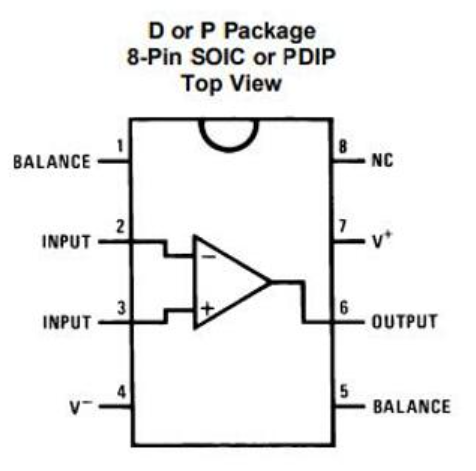
\includegraphics[scale=0.33]{pinout.png}
    \caption{\textit{LF365N} pin schematic }
    \label{fig:91}
\end{figure}

From here, the pins 1 and 5 are not used in the actual experiment, and the labels $V+,V-$ will correspond to $V_{ss}$ and $V_{cc}$ respectively.

\section{Results}

\subsection{Simulating the superposition principle}

With \textit{LTSpice}, the following schematic was built

\begin{figure}[h]
    \centering
    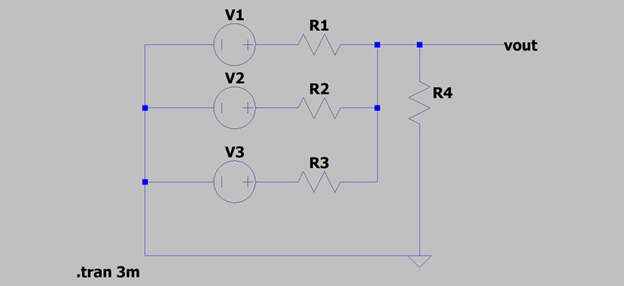
\includegraphics[scale=0.8]{exp1-circuit.png}
    \caption{\ltspice simulation for superposition}
    \label{fig:9}
\end{figure}

When turning $v_2,v_3$ of, the following graph was produced

\begin{figure}[h]
    \centering
    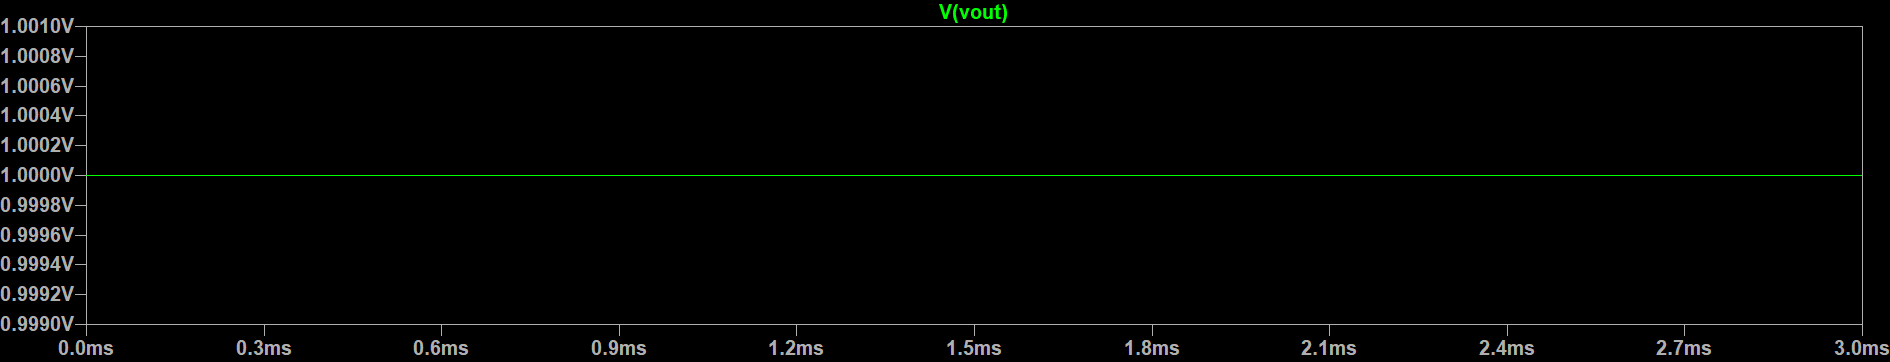
\includegraphics[scale=0.25]{exp1-v1.png}
    \caption{Simulation with only the first source on}
    \label{fig:10}
\end{figure}

\newpage
With only $v_2$ on

\begin{figure}[h]
    \centering
    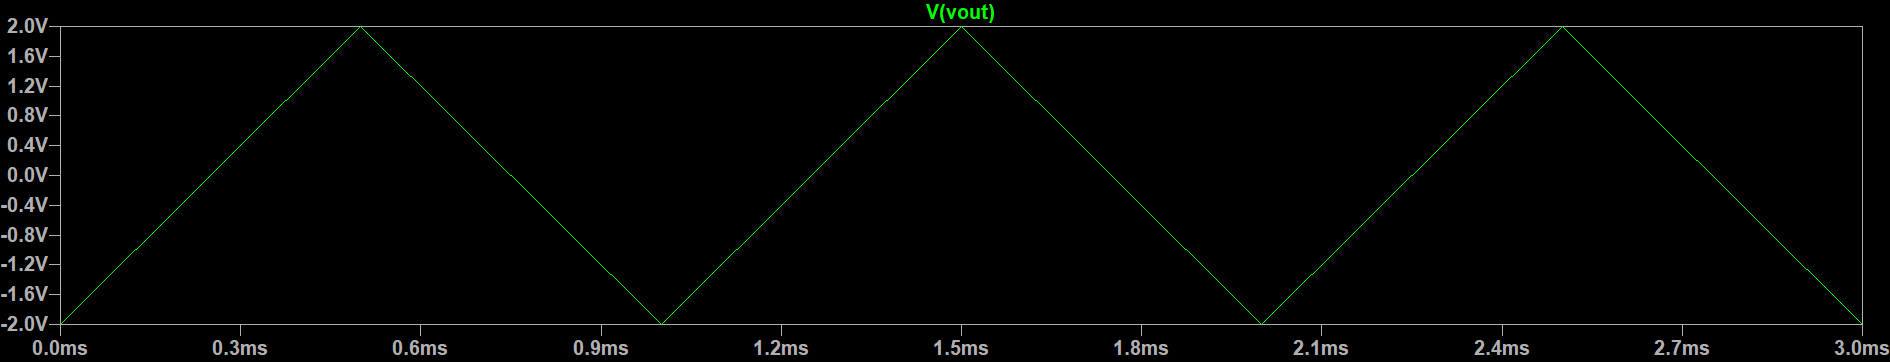
\includegraphics[scale=0.25]{exp1-v2.png}
    \caption{Simulation with only the second source on}
    \label{fig:11}
\end{figure}

With only $v_3$

\begin{figure}[h]
    \centering
    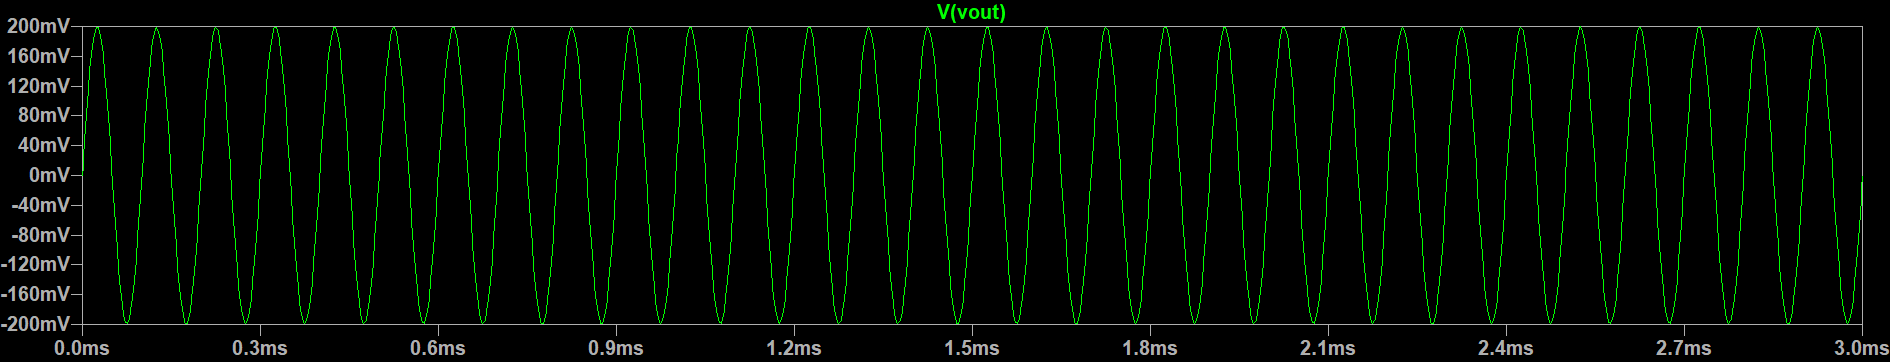
\includegraphics[scale=0.25]{exp1-v3.png}
    \caption{Simulation with only the third source on}
    \label{fig:12}
\end{figure}

Finally, the last simulation with all the sources on

\begin{figure}[h]
    \centering
    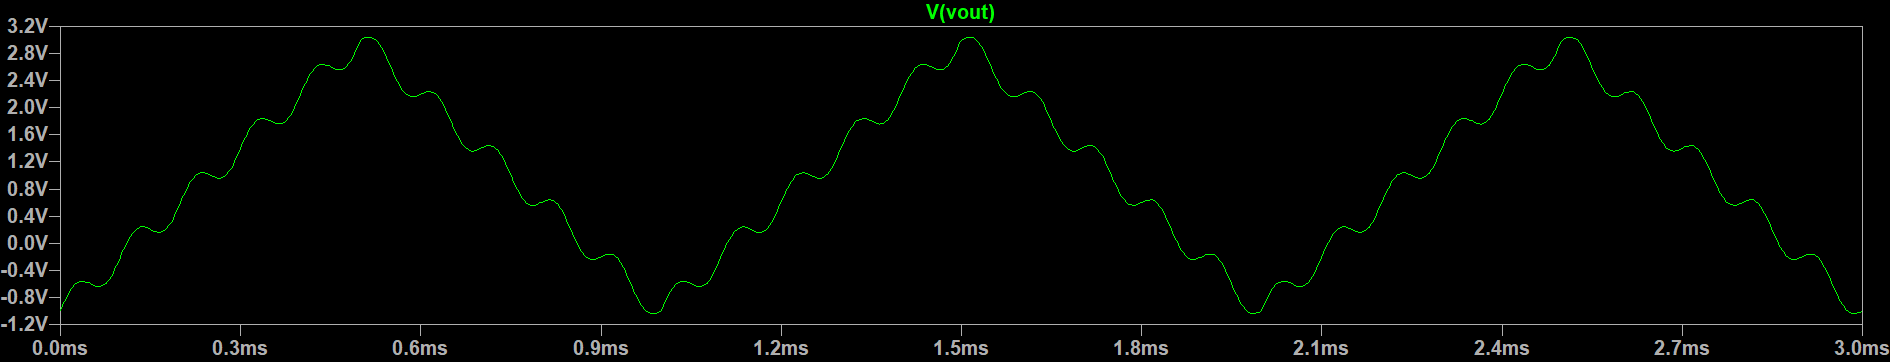
\includegraphics[scale=0.25]{exp1-all.png}
    \caption{Simulation with all sources on}
    \label{fig:13}
\end{figure}

From this results, we can verify the superposition principle, since the graph of figure (\ref{fig:13}) is the same as adding figure (\ref{fig:10}), (\ref{fig:11}), and (\ref{fig:12}). For example, note that $V_{\text{peak}}$, or the peak voltage, would be

\begin{align*}
    V_{\text{peak}} &= \underbrace{\SI{1}{\volt}}_{\text{Peak of source 1}} + \underbrace{\SI{2}{\volt}}_{\text{Peak of source 2}}+ \underbrace{\SI{200}{\milli\volt}}_{\text{Peak of source 3}}\\
    \Aboxed{V_{\text{peak}} &= \SI{3.2}{\volt}.}
\end{align*}

Which is the same peak as the one of Figure (\ref{fig:13}).

Another approach to this result is that the voltage at a time $t$ $V(t)$ can be expressed as the linear sum of each of the sources multiplied by a constant, remember Equation (\ref{eq:3})

\begin{align*}
    V(t) &= \alpha V_\text{Source 1} + \beta V_\text{Source 2} + \gamma V_\text{Source 3}
\end{align*}

Where $\alpha,\beta,\gamma$ are constants.

To find such constant we can take advantage of the results when only one of the sources was on, for example
 \begin{align*}
    V_\text{out, source 1} &= \alpha V_\text{Source 1}\\
     \SI{1}{\volt} &= \alpha \SI{2.25}{\volt}\\
     \Aboxed{\alpha &= 0.4444.}
 \end{align*}

 A similar process can be done to get

 \begin{align*}
     \Aboxed{\beta &= 0.4444}\\
     \Aboxed{\gamma &= 0.0556}
 \end{align*}

 Such that the final equation for $V(t)$ is
 \begin{align*}
    V(t) &= (0.4444)\SI{2.25}{\volt} + (0.4444)4.5tri(2\pi1000t) \SI{}{\volt} + (0.0556)3.6\sin(2\pi10000t) \SI{}{\volt}\\
     V(t) &= \SI{1}{\volt} + 2tri(2\pi10000t) \SI{}{\volt} + 200\sin(2\pi10000t) \SI{}{\milli\volt}.
 \end{align*}
 \newpage
\subsection{Thévenin equivalent circuit design and generalizing a procedure to find Thévenin equivalent}

First we need to design the circuit, to get this, multiple source transformations were done so the initial circuit transforms into
\begin{figure}[h]
\begin{subfigure}{.5\textwidth}
        \centering
        \begin{circuitikz}[]
        \draw (6,0) to [short, o-*](3,0) to [short](0,0) to [V,l=$V_s$,invert](0,4) to [R,l=$R_1$,-*](3,4) to [R,l=$R_3$,-o](6,4) ;
        \draw (3,0) to [R,l=$R_2$](3,4) ;
        \draw (6,0) to [open, v_<= $v_{\text{out}}$](6,4) ; 
    \end{circuitikz}
    \caption{Circuit to build}
\end{subfigure}
\begin{subfigure}{.5\textwidth}
        \centering
        \begin{circuitikz}
            \draw (4,0) to [short,o-](0,0) to [V, l=$\frac{V_s}{R_1}(R_1||R_2)$,invert](0,4) to [R, l =$(R_1||R_2) + R_3$, -o](4,4);
            \draw (4,0) to [open,v<= $v_\text{out}$](4,4) ;
        \end{circuitikz}
    \caption{Circuit After source transformations}
\end{subfigure}
\caption{Circuit analysis to calculate equivalent circuit}
\end{figure}

Note that the Thévenin voltage $V_{th}$
\begin{align*}
    V_{th} &= v_{\text{out}}\\
    V_{th} &= \frac{V_s}{R_1}(R_1||R_2) = \SI{2.5}{\volt}
\end{align*}

And the equivalent resistance $R_{eq}$
\begin{align*}
    R_{eq} &= (R_1||R_2) + R_3 = \SI{1.5}{\kilo\ohm}
\end{align*}

Note that the system has 4 unknowns and 2 equations, so there are infinite solutions. Nonetheless, the goal is to get simple numbers that we can find in the lab kit in order to build the circuit. After some trial and error, $R_1 = R_2 = \SI{1}{\kilo\ohm}$ was found to be a good choice. With that in mind

\begin{align}
    R_1 ||R_2 = \SI{500}{\ohm} \label{eq:4}
\end{align}

Using equation (\ref{eq:4}) into the $V_{th}$ expression

\begin{align*}
    \SI{2.5}{\volt} &= \frac{V_s}{\SI{1}{\kilo\ohm}} \SI{500}{\ohm}\\
    \SI{2.5}{\volt} &= \frac{V_s}{2}\\
    V_s &= \SI{5}{\volt}.
\end{align*}

And in the equivalent resistance equation

\begin{align*}
    (R_1||R_2) + R_3 &= \SI{1.5}{\kilo\ohm}\\
    R_3 &= \SI{1}{\kilo\ohm}
\end{align*}

Which leads to the following solution

\begin{align*}
\boxed{
\begin{array}{rcl}
V_s &= \SI{5}{\volt} \\
R_1 = R_2 = R_3 &= \SI{1}{\kilo\ohm}
\end{array}
}
\end{align*}

With the values calculated, the circuit was built, find the picture below 

\begin{figure}[h]
    \centering
    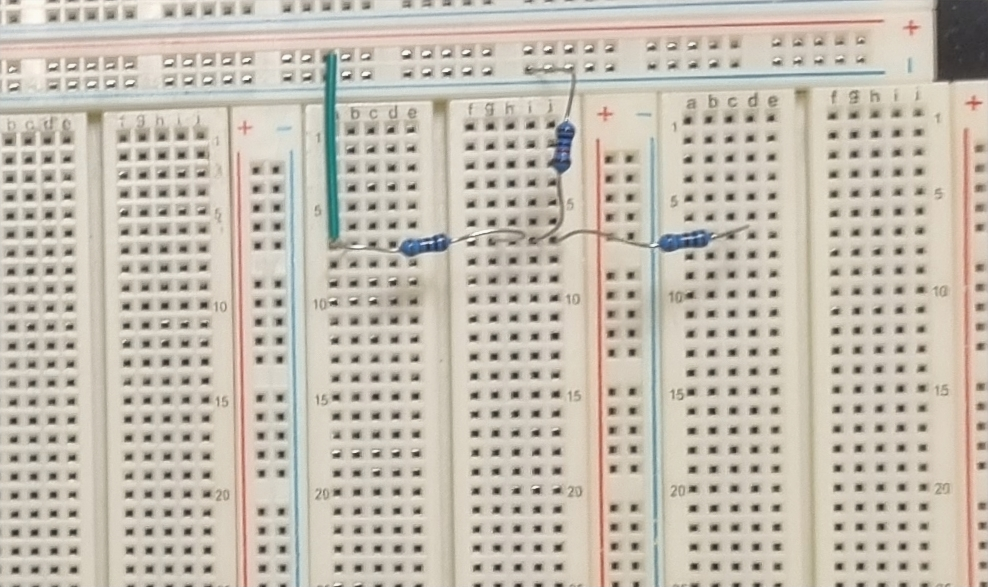
\includegraphics[scale=0.35]{20221012_202819.jpg}
    \caption{Circuit build for experiment 2}
    \label{fig:16}
\end{figure}

For the general procedure, the following method was developed

\begin{enumerate}
    \item Locate the two ports used to calculate the equivalent circuit
    \item Measure the voltage across them by connecting a voltmeter, this will be $V_{th}$
    \item Measure the current across the two ports with an ammeter
    \item Calculate the equivalent resistance by dividing the value from the voltmeter by the current, this will be $R_{eq}$
\end{enumerate}

Applying this method to the circuit, the reuslts were

\begin{align*}
    V_{th} &= \SI{2.486}{\volt}\\
    I_{nt} &= \SI{1.66}{\milli\ampere}\\
    \therefore\\
    R_{eq} &= \SI{1479}{\ohm}.
\end{align*}

Comparing these results with the theoretical ones

\begin{table}[h]
    \centering
    \begin{tabular}{|c|c|}
    \toprule
         Value measured& \%Error  \\
         \midrule
        $V_{th} = \SI{2.486}{\volt}$ & 0.56\%\\
        $R_{eq} = \SI{1479}{\ohm}$ & 1.4\%\\
        \bottomrule
    \end{tabular}
    \caption{Results of the designed circuit}
    \label{tab:2}
\end{table}

\subsection{Implementation of a voltage buffer to reduce the load of the waveform generator}

The circuit in Figure (\ref{fig:6}) was built, when the waveform was turned on the following results where obtained for $V_{RMS}$

\begin{table}[h]
    \centering
    \begin{tabular}{|c|c|c|}
    \toprule
         Theoretical $V_{RMS}$& Measured $V_{RMS}$ & \% Error\\
         \midrule
         $V_{RMS} = \frac{A}{\sqrt{2}} \approx \SI{0.17}{\volt}$& \SI{0.028}{\volt} & 87.5\%\\
         \bottomrule
    \end{tabular}
    \caption{Results of the first circuit in experiment 3}
    \label{tab:3}
\end{table}
\newpage
This results indicate the presence of some load, since if the circuit was just like the one described in the procedure, the error should not be as big. This is probably because there is a load of the source not accounted for, meaning that the actual circuit would be some of the form

\begin{figure}[h]
    \centering
    \begin{circuitikz}
        \draw (0,0) to [sV, v<={$V_s$}](0,4) to [R,l=$R_s$](4,4) to [generic, l=Speaker,v = $V_{\text{speaker}}$](4,0) to [short](0,0);
    \end{circuitikz}
    \caption{Initial schematic for speaker-waveform circuit with load}
    \label{fig:16}
\end{figure}

Where $R_s$ is an associated load of the waveform.

The second circuit in Figure (\ref{fig:7}) was built. During this construction, all the system shared a common ground node and multiple problems with the cables connections arose, but after trouble shouting and changing cables, the following results were 
obtained for $V_{RMS}$.

\begin{table}[h]
    \centering
    \begin{tabular}{|c|c|c|}
    \toprule
         Input voltage $V_{in}$& Output Voltage $V_{\text{out}}$&  \% Difference \\
         \midrule
         \SI{0.17646}{\volt}& \SI{0.15393}{\volt} & 12.7768 \%\\
         \bottomrule
    \end{tabular}
    \caption{Results of the circuit with the op amp}
    \label{tab:4}
\end{table}

The results show the effect of the voltage buffer, since the effect of the load in the waveform generator got reduced by a significant amount. 
\newpage
Now, in order to estimate the equivalent circuit, lets consider the following circuit

\begin{figure}[h]
    \centering
    \begin{circuitikz}
        \draw (0,0) to [sV, v<= $V_{in}$] (0,4) to [R, l = $R_{th}$] (4,4) to [generic, a=$\SI{8}{\ohm}$] (4,0)  to [short](0,0);
        \draw (4,4) to [short, -o](5,4) node[] (+sign) ;
        \draw (4,0) to [short,-o] (5,0) node[] (-sign) ;
        \draw (-sign) to [open,v<=$V_{out}$](+sign) ;
    \end{circuitikz}
    \caption{Equivalent circuit for experiment 3 }
    \label{fig:my_label}
\end{figure}

Using the calculated values, a trivial computation follows (voltage division)

\begin{align*}
    V_{out} &= V_{in} \frac{\SI{8}{\ohm}}{ \SI{8}{\ohm} + R_{th}}\\
    R_{th} &= \frac{V_{in}\SI{8}{\ohm}}{V_{out}} - \SI{8}{\ohm}\\
    R_{th} &= \frac{\SI{0.17646}{\volt}\cdot\SI{8}{\ohm}}{\SI{0.15393}{\volt}} - \SI{8}{\ohm}\\
    \Aboxed{R_{th} &\approx \SI{1.17092}{\ohm}.}
\end{align*}

\newpage
\section{Conclusion}

In this report, powerful concepts of Electrical Engineering were checked and understood, by verifying the superposition principles and Norton Equivalent theorem, I can now apply the knowledge to virtually any linear circuit. These two concepts merged into the final experiment, where an equivalent circuit was built. Overall, all the objectives were accomplished since the theorems were verified.

Finally, the understanding of how an op amp or voltage buffer works is a key concept, since the over-simplified models presented in theory are not always enough to produce a practical result. In these scenarios, knowing how to use the voltage buffer to reduce the load of the source is a major concept to understand.

\newpage
\printbibliography
\end{document}